\section{Software}



\subsection{Development Software}

Several software packages were used to implement and test the trigger logic developed for CLAS12. These were the FPGA synthesis and implementation and FPGA high level synthesizer.

For FPGA synthesis and implemenation Xilinx ISE/Planahead and Vivado were used. Most of the front-end boards were developed years ago and use Virtex 5 and Spartan 6 FPGAs, which are not supported by Xilinx Vivado, so we relied on Xilinx ISE/Planahead for synthesis and implementation. Even though these tools are no longer updated by Xilinx they have proved to be stable, reliable, and deliver consistent results. Newer design use Xilinx 7-series parts (we used Artix, Kintex, and Virtex) so we used the Vivado tools, which had far better support than ISE/Planahead.

Vivado HLS was used to implement a variety of trigger algorithms, event builder logic, and general purpose logic. HLS components were able to be verified with C/C++ test benches on their own without anything more than GNU GCC and associated C/C++ header files from the HLS toolchain. This tool often allowed for faster implementation for FPGA implemenation, but many components still were implemented in HDL were resource and/or timing requirements become critical. Vivado HLS generated VHDL files from the C/C++ sources that were included into the FPGA compilation and full simulations. Occasionally simulation of the HDL generated files was required to debug C/C++ modules when simulation under GCC found no problem, but the HDL result did. Differences between C/C++ simulation and the corresponding HDL output were primarily due to: C/++ assumption of infinite length buffering while HDL buffers were finite, ambiguous C/C++ coding where GCC and HLS behaviors differed, and latency issues due to the C/C++ simulation has no concept of elapsed time.

\subsection{Operating Systems} Moffit

Linux operating systems are used on all readout controllers in the CLAS12 DAQ. The VME crate controllers use Intel based CPUs and run a standard Centos and Linux kernel distribution. The VTP modules use an ARMv7 CPU with custom hardware and run Arch Linux using a custom Linux kernel. Both CPUs boot from the network using a shared kernel and root filesystem images, which simplify administration. Common DAQ software (readout, configuration, slow control, diagnostics, etc.) tools are able to used for both platforms and most tools available on standard desktop PCs are also available to use.

Archlinux with armv7

\begin{itemize}
\item Linux Kernel 4.4.0
  \begin{itemize}
  \item Updates with specific support for Xilinx Zynq Processors
  \item Available at https://github.com/Xilinx/linux-xlnx.git
  \item Custom device-tree
  \item Provides FPGA programming interface
  \item Allocates Physical Memory for use with DMA and event buffers
  \item Standard I$^2c$ and SPI API
  \end{itemize}

\item Archlinux compiled for armv7
  \begin{itemize}
  \item Available at https://archlinuxarm.org/
  \item Filesystem over NFS
  \item diskless booting using tftp (UBoot)
  \end{itemize}
\end{itemize}


\subsection{Configuration Software}

\subsubsection{Configuration Files} sergey

CLAS12 Trigger system has large amount of parameters controlling its logic. Those parameters are set by writing values to hadrware registers, and controlled by reading those registers back. System is using ascii files, example is shown on (Fig.). Every line contains key word and the number of corresponding parameter values. Directive 'include' allows to use hierarhical set of configuration files. Normally main configuration file is selected during run startup procedure, and run control software resolves all 'include' directives creating one big configuration file. That file is used to program all trigger harwdare registers, and it is also written to the data stream for bookkeeping purposes. Register contents are read back and results recorded into data stream as well, providing full control of trigger system settings. Normally the same configuration files contains DAQ settings as well, makeing it complete source for entire DAQ/Trigger system settings.


\subsubsection{Timing Setting}

\begin{figure}[hbt]
	\centering
	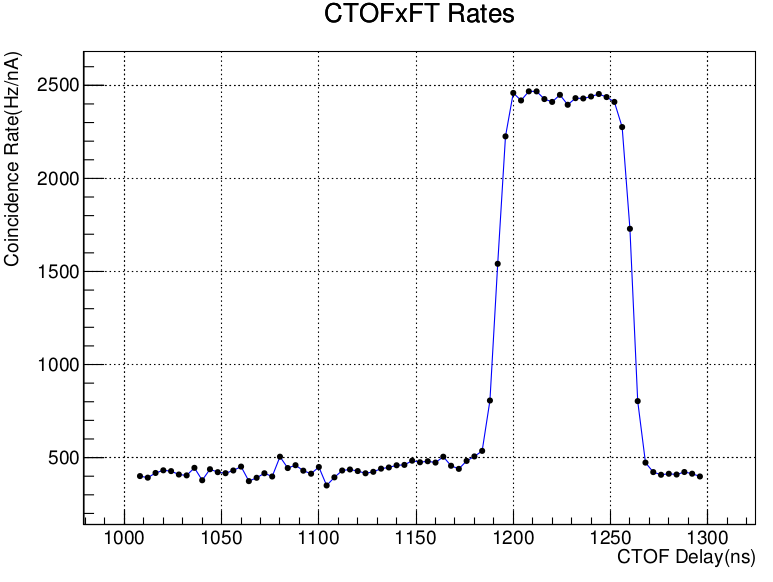
\includegraphics[width=1.0\columnwidth,keepaspectratio]{img/delay_scan_ctof_ft.png}
	\caption{CTOFxFT Delay Scan}
	\label{fig:delay_scan_ctof_ft}
\end{figure}

One of the important components of the trigger setting process is delay curves measurements. For that purpose software procedure was developed. It includes special trigger configuration file and software tools to sweep individual subsystem latencies, record set of beam current normalized scalers, and produce corresponding delay plots Fig.~\ref{fig:delay_scan_ctof_ft}. Time trigger time setting detector was kept at a constant value, which determined the DAQ readout window timing, while the other subsystems were changed step by step to monitor the delay curve. Delays and coincidence widths were adjusted to account for known jitter sources to ensure no events are lost due poor timing alignment. This procedure was repeated every time trigger logic was changed.


\subsubsection{Gain calibration and Threshold settings}

One of the important settings in trigger system is FADC ones. As it stated above FADC boards serves as initial stage of the most of the Stage 1 trigger components (except Drift Chamber), and correct pedestal and gain calibration is critical for correct trigger system performance. Pedestal and gain measurements were conducted before run startup, and values were loaded using configuration files. As result, all thresholds in configuration files were set using understandable units such as MeV for calorimeters and the number of photoelectrons for cherenkov counter.
